
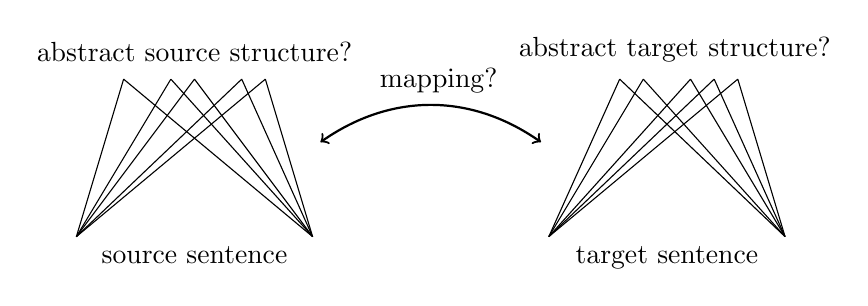
\begin{tikzpicture}

\coordinate (ss) at (1.5,0);
\node [below] at (ss) {source sentence};

%\draw[] (0,0) -- node[below]{source sentence} (3,0);
\draw (0,0) -- (0.6,2) (3,0) -- (0.6,2);
%\draw (0,0) -- (0.9,2) (3,0) -- (0.9,2);
\draw (0,0) -- (1.2,2) (3,0) -- (1.2,2);
\draw (0,0) -- (1.5,2) (3,0) -- (1.5,2);
%\draw (0,0) -- (1.8,2) (3,0) -- (1.8,2);
\draw (0,0) -- (2.1,2) (3,0) -- (2.1,2);
\draw (0,0) -- (2.4,2) (3,0) -- (2.4,2);

\node [above] at (1.5,2.1) {abstract source structure?};
\node [above] at (4.6,1.7) {mapping?};
\node [above] at (7.6,2.1) {abstract target structure?};
\coordinate (ts) at (7.5,0);
\node [below] at (ts) {target sentence};

%\draw (6,0) -- (0.6,2) (9,0) -- (6.6,2);
\draw (6,0) -- (6.9,2) (9,0) -- (6.9,2);
\draw (6,0) -- (7.2,2) (9,0) -- (7.2,2);
%\draw (6,0) -- (7.5,2) (9,0) -- (7.5,2);
\draw (6,0) -- (7.8,2) (9,0) -- (7.8,2);
\draw (6,0) -- (8.1,2) (9,0) -- (8.1,2);
\draw (6,0) -- (8.4,2) (9,0) -- (8.4,2);

\coordinate (startarrow) at (3.1,1.2);
\coordinate (endarrow) at (5.9,1.2);

\draw[<->,bend left =35, thick] (startarrow) to (endarrow);

\end{tikzpicture}
